\documentclass{scrartcl}
\usepackage{hyperref}
\usepackage[utf8]{inputenc}
\usepackage{graphicx}
\usepackage{cite}
\usepackage{amssymb}
\usepackage{amsmath}
\graphicspath{{./images/}}
\hypersetup{
    colorlinks=true,
    linkcolor=blue,
    filecolor=magenta,      
    urlcolor=cyan,
}
\urlstyle{same}
\title{Neural Networks in Text Processing}
\subtitle{ Natural Language Processing }
\date{06-01-2020}
\author{Fernando André Bezerra Moura Fernandes - bez0070}

\begin{document}
    \maketitle
    \pagenumbering{gobble}
    \newpage
    \tableofcontents
    \newpage
    \pagenumbering{arabic}
    \section{ Abstract }
    \textbf{Text Processing} allows the automation of creating and manipulating electronic text 
    with numerous modern applications such as grammar and spell checking, text completion,
    plagiarism detection or even chat bots. Thus, the theory behind text processing techniques
    requires a lot of \textbf{algorithmic} and \textbf{data structure} knowledge. \newline
    These techniques allow the development of artificial intelligence applications and with
    normally have to deal with large quantities of strings when analyzing textual documents
    for their different uses. \newline
    One very specific use case of textual analysis is \textbf{Natural Language Processing} 
    which is the one of the two main topics of this document. \newline
    \textbf{Natural Language Processing} is an artificial intelligence field concerned with 
    interactions between computers and a language and (i.e English) and the
    processing of textual data in that language so that the machine can make
    conclusions about that document. \newline
    In order to understand a document written in some language a computer program must first
    pre-process that document so that later it can be modeled in a computable way. 
    Common ways of doing this include:
    \begin{itemize}
        \item \textbf{Tokenizing the document} by breaking down the document's text into 
        different words and representing a document in memory by its words. One example is to
        divide the document by the space character and getting the words that way.
        \item \textbf{Stemming the words} which means to get the base word and removing the 
        derivational affixes.  
        \item \textbf{Lemmatization} by removing the inflectional ending of the words and getting
        the root word ensuring it belongs to that language.
        \item \textbf{N-Grams}. N-grams refer to the process of combining the nearby words 
        together for representation purposes where N represents the number of words to be 
        combined together.
    \end{itemize}
    In order to model a document by its content, first a meaning must be given to the words it
    contains. \newline 
    One way of doing this calculating a \textbf{TF-IDF} value for each word on a
    document, which can be interpreted as its weight. Another way would be calculating
    \textbf{One-Hot Encodings} or \textbf{Word Embeddings} which are other ways 
    of representing words in a document.
    After these transformations the document can be represented in a certain format
    such as a \textbf{Bag of Words}. \newline 
    All these concepts and techniques and much more are used by \textbf{Deep Neural Networks} in 
    the field of Natural Language Processing. \textbf{Neural Networks} are a set of algorithms 
    which are modeled to resemble the way that the human brain works. Deep Neural Networks
    are a subfield of Neural Networks which use multiple layers to progressively extract 
    higher level features of the input they are given. \textbf{DNN} have revolutionized the field
    of Natural Language Processing and are the second main topic of this document. 
    \newpage
    \section{ Introduction }
    Neural networks in the area of computer science are mostly refered to as 
    \textbf{Artificial Neural Networks} and are based on the neural structure of the brain,
    being able to learn to perform tasks such as classification and clustering. \newline
    An ANN consists of a series of nodes, which are interpreted as artificial neurons which
    are part of a directed and weighted graph and can be set on an input layer, 
    output layer, or on the middle hidden processing layer or layers.
    
    \begin{figure}[h!]
        \centering
        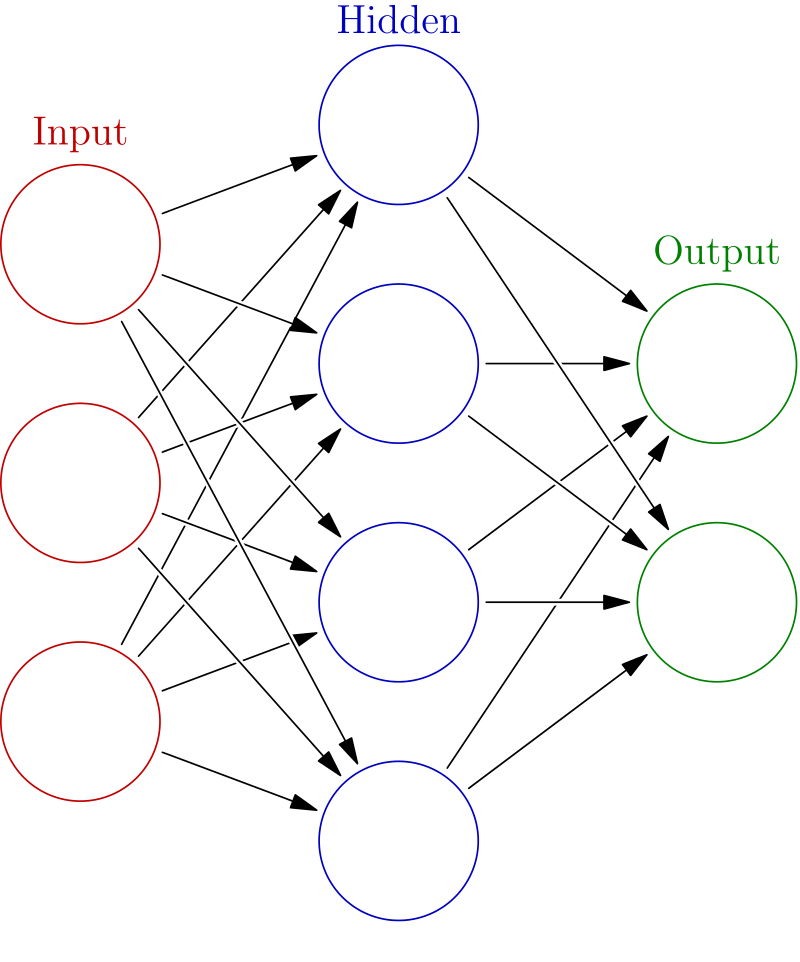
\includegraphics[scale=0.2]{ann.png}
        \caption{A representation of an ANN}
    \end{figure}
    The input layer receives input, parses it and sends information to the hidden layer(s) which
    in turn sends it to the output layer. Every neuron(node) has \textbf{synapses}(input), 
    which they combine with their internal state using an \textbf{activation function} and produce
    an output. The input to a neuron is the output of other neurons or simply another neuron,
    which is computed by a \textbf{propagation function}.
    An ANN also possesses \textbf{hyperparameters} which are parameters who controll the network,
    are set before the learning process and change according via learning. Examples of these 
    parameters include the \textbf{learning rate} or the number of hidden layers and can depend
    on other hyperparameters. \newline
    The ANN consumes a dataset, considering it as a sample observation and uses one part of 
    the dataset(train) to be trained and to learn, varying its hyperparameters and another part 
    (test) to check its accuracy. 
    \textbf{Learning} involves adjusting the weights of the network 
    to decrease an error rate. Usually this \textbf{error rate} is divided among the connections and 
    \textbf{backpropagation} is used to adjust the connection weights. Backpropagation is a method
    who calculates the \textbf{gradient} of the \textbf{cost function}(which measures the performance
    of the ANN regarding its test set) and then the weight updates are often performed using
    \textbf{stochastic gradient descent} or other methods.
    Depending on their internal organization, or the way they change their weights there are many
    different types of ANN, and throughout the rest of this research document, their uses on
    Natural Language Processing will be described.
    \section{ Deep Learning on Natural Language Processing }
    Depending on the NLP task at hand we can use different artificial neural network models and
    achieve different results.
    First we must discuss to how features in a document should be represented. \newline
    Generally speaking, in NLP the sparse-input encodes features such as words
    or part-of-speech tags. The initial task is to parse this input into a neural-network
    base model and start representing each feature as a \textbf{dense vector}. 
    Each feature is \textbf{embedded} into a dimensional space, and represented as a vector in 
    that space, and is treated as a model parameter which needs to be trained together 
    with other components of the network.
    One benefit of using dense and low-dimensional vectors is computational since
    the majority of neural network toolkits do not play well with very high-dimensional, sparse  
    vectors. The other benefit of the dense representations is in generalization power because 
    as some features may provide similar clues, it is worthwhile to provide a representation that
    is able to capture these similarities. \newline
    In cases where we have relatively few distinct features in the category, and we believe
    there are no correlations between the different features,
    we may use the one-hot representation vectors.
    The one-hot representation vectors result in a sparse feature vector where each dimension
    is a feature and feature combinations receive their own dimension, and where values inside
    the vector are binary resulting in high dimensionality. Dense feature representations,
    represent each feature as a vector resulting in low dimensionality and the feature-to-vector
    mapping is made on an \textbf{embedding matrix}. 
    There is also another problem with features related with the number in which they occur, as 
    in some cases their number is not known in advance. Thus, an unbounded 
    number of features needs to be represented using a fixed size vector. One way of doing this
    is using a \textbf{continuous bag of words}. The traditional bag of words 
    is a way to represent the data in a tabular format with columns representing the 
    total vocabulary of the documents, rows representing a single observation and each cell
    being filled up by the observation frequency.
    The CBOW is very similar to the traditional bag-of-words representation in which
    we discard order information, and works by either summing or averaging the 
    embedding vectors of the corresponding features.
    \begin{equation}
        CBOW(f_1, ...., f_k) = \frac{1}{k} \sum^{k}_{i=1}v(f_i)
    \end{equation}
    Now, we will describe a series of different neural network architectures and the way they
    are using on NLP tasks.
    \newpage
    \subsection{Feed Forward Neural Networks}
    A \textbf{feed forward neural network} is an acyclic type of neural network architecture, 
    which means the connections between the nodes do not form any cycles in the whole network.
    \begin{figure}[h!]
        \centering
        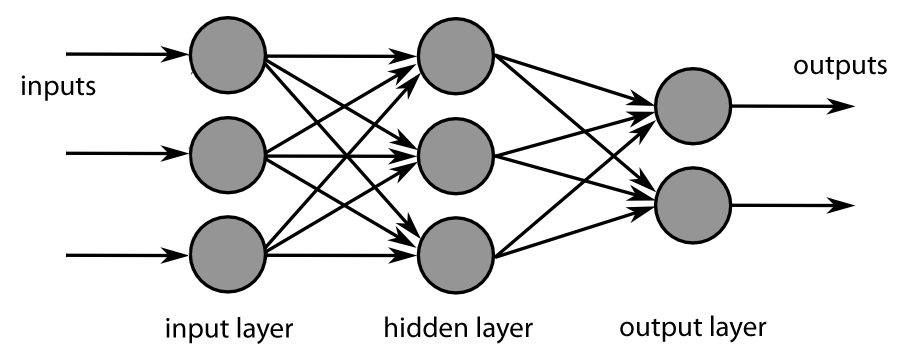
\includegraphics[scale=0.4]{ffnn.png}
        \caption{A representation of a Feed Forward Neural Network}
    \end{figure} \newline
    As we can see from figure 2 the information is carried always in one direction from the 
    input to the output.
    Using mathematical notations, each layer in the network implements a vector-matrix
    multiplication $\textbf{h = xW}$ where \textit{W} represents the weights matrix and 
    \textit{x} represents the layer vector(nodes in that layer). The values of \textit{h}
    are then transformed using a linear function \textit{g} before being passed to the next layer.
    We define the whole computation as follows: $g(xW_1)\prod^n_{i=2}W_i$, where \textit{n} 
    is the number of hidden layers and \textit{$W_i$} represents the weight matrix of the ith 
    layer.
    \subsubsection{ Multi Layer Perceptron }
    A \textbf{Multi Layer Perceptron} is a class of feed forward neural networks and its
    architecture is composed of multiple layers of \textbf{perceptrons}. Perceptrons are
    the simplest neural network and are considered binary classifiers whose algorithm 
    is based on a linear prediction function. \newline
    \begin{equation}
        Perceptron(x) = xW + b
    \end{equation}
    The term \textit{b} is the bias.
    The multi layer perceptron is able to go beyond linear functions by adding more perceptron
    layers.
    Example with 2 hidden layers:
    \begin{equation}
        MLP_2(x) = (g_2(g_1(xW_1 + b_1)W_2 + b_2))W_3
    \end{equation}
    The vector resulting from each linear transform is referred to as a layer. 
    The outer-most linear transform results in the output layer and the other linear transforms 
    result in hidden layers. Each hidden layer is followed by a non-linear activation.
    \newpage
    In an NLP application, \textit{x} is normally composed of embedding vectors, wether they 
    are one-hot representations or dense representations.
    One common task in NLP is classification, and one frequently used method used in text
    classification is the multilayer perceptron.
    \begin{figure}[h!]
        \centering
        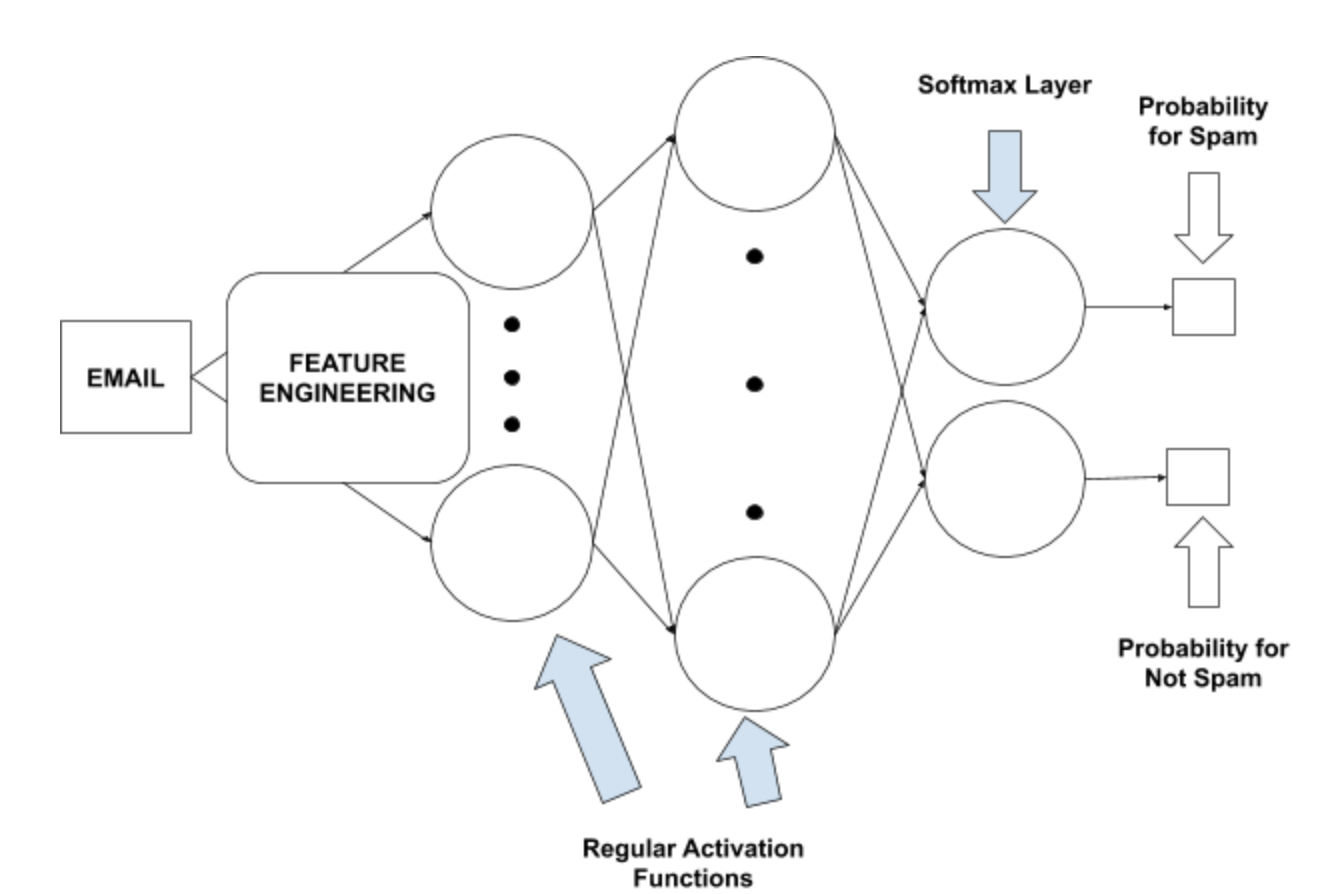
\includegraphics[scale=0.2]{mlp.png}
        \caption{Email spam classification with a MLP}
    \end{figure} \newline
    \newline
    First, a set of features are derived from an e-mail text, which are feeded to an input
    layer and then results from that layer are propagated into the hidden middle layers.
    In this case the output layer will yield a size 2 vector with probabilities for the 
    \textit{Spam} and \textit{Not spam} classes.
    The \textbf{Softmax Layer} contains a series of neurons whose activation function is
    the softmax function which converts a set of class scores into equivalent class
    probabilities.
    \begin{equation}
        \sigma(x)_j = \frac{e^{xj}}{\sum^k_{i=1} e^{xi} }
    \end{equation}
    \newpage
    \subsubsection{Convolutional Neural Networks}
    \begin{figure}[h!]
        \centering
        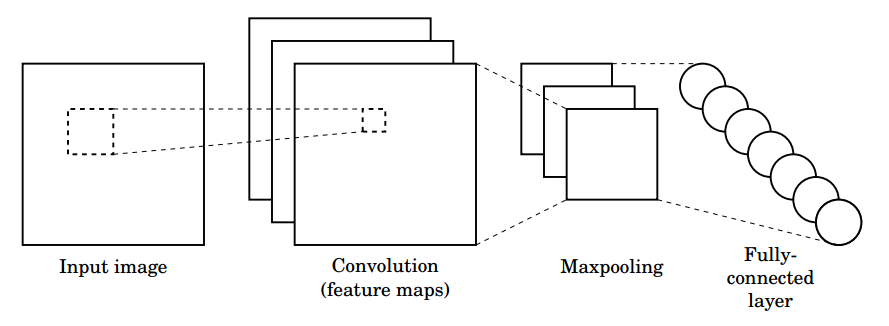
\includegraphics[scale=0.4]{cvnn.png}
        \caption{Representation of a CNN}
    \end{figure} 
    \textbf{Convolutional Neural Networks} use \textbf{convolution} in place of matrix
    multiplication on at least on of their layers. \newline
    The hidden layers of a CNN typically consist of a series of convolutional layers 
    that convolve with a multiplication or other dot product. 
    The activation function is commonly a \textbf{rectifier} layer, 
    and is subsequently followed by  additional convolutions such as \textbf{pooling} layers, 
    \textbf{fully connected layers} and \textbf{normalization} layers, 
    referred to as hidden layers because their inputs and outputs are masked by the activation 
    function and final convolution. The final convolution, in turn, often involves 
    backpropagation in order to more accurately weight the end product.
    Convolution  is a mathematical operation on two functions that produces a 
    third function expressing how the shape of one is modified by the other.
    On the previous section, when describing the MLP model, the e-mail spam classifier
    was mentioned. On this section we will make reference to a papper, 
    \textit{"Deep Convolutional Neural Networks for Sentiment Analysis of Short Texts"}
    \cite{dos-santos-gatti-2014-deep}, on which the authors propose a convolutional
    neural network architecture for a NLP task which extracts sentiment analysis when analyzing
    textual data.
    Their proposed deep neural network is called \textbf{CharSCNN}, 
    \textit{Character to Sentence Convolutional Neural Network}, and uses 2 convolutional layers
    to extract relevant features from words and sentences of any size. They focus their work 
    on small textual data, such as movie reviews or Twitter messages. 
    Given a sentence, the network computes a score for each sentiment label. 
    In order to score a sentence, the network takes as input the sequence of words in the sentence, 
    and passes it through  a sequence of layers where features with increasing levels of 
    complexity are extracted.
    The first layer of the network transforms words into real-valued feature vectors (embeddings) 
    that capture morphological, syntactic and semantic information about the word.
    The sentences are represented using a set of N words ${w_1, w_2, w_3, ..., w_n}$ and every
    word $w_n$ is converted into a vector $u_n = [r^{wrd}, r^{wch}]$. The first element of the 
    vector is the \textbf{word-level embedding} and the second one is the 
    \textbf{character level-embedding}.
    Word-level embeddings are encoded by column vectors in an embedding matrix 
    $W^{wrd} \in \mathbb{R}^{d^{wrd} \times | V^{wrd} | }$
    The word is transformed into irs word-level embedding by:
    \begin{equation}
        r^{wrd} = W^{wrd}v^{w}
    \end{equation}
    \newpage
    For character-level embedding, considering a word to be represented by M characters
    ${c_1, c_2, c_3, ..., c_m}$ the character embedding is:
    \begin{equation}
        r^{chr} = W^{chr}v^c
    \end{equation}
    $W^{chr} \in \mathbb{R}^{d^{chr} \times | V^{chr} | } $ is the character embedding matrix.
    They define the next step in CharSCNN to be extracting a sentence-level representation
    $r^{sent}_x$.
    The second convolutional layer produces local features around each word in the sentence
    and then combines them using a \textit{max} operation to create fixed-sized feature
    vectors for the word sequence(sentence). The network is trained by minimizing
    a negative likelihood over a training set. \newline
    This is just an example of how CNN's can be used for NLP tasks.
    \subsection{ Recurrent Neural Networks }
    \textbf{Recurrent Neural Networks} is a variant of \textbf{recursive neural networks}
    characterized by being a directed cyclic graph. They use their internal state, stored
    in memory, to process sequences of inputs, being extremely useful for cases where
    input order matters, like in most NLP applications.
    \begin{figure}[h!]
        \centering
        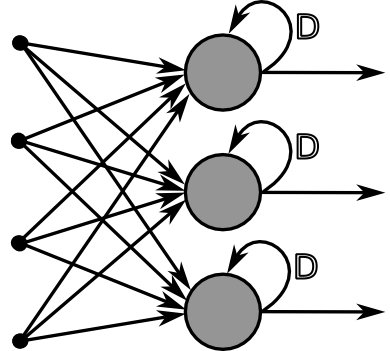
\includegraphics[scale=0.4]{rnn.png}
        \caption{Representation of the RNN's recurrent layer}
    \end{figure} 
    In \textit{"Recurrent Neural Networks for Language Understanding"} \cite{rnn-lu}, 
    the authors use a RNN architecture for LU tasks such as labeling words with semantic
    meaning. They use the classic \textbf{Elman} architecture for this purpose.
    \begin{figure}[h!]
        \centering
        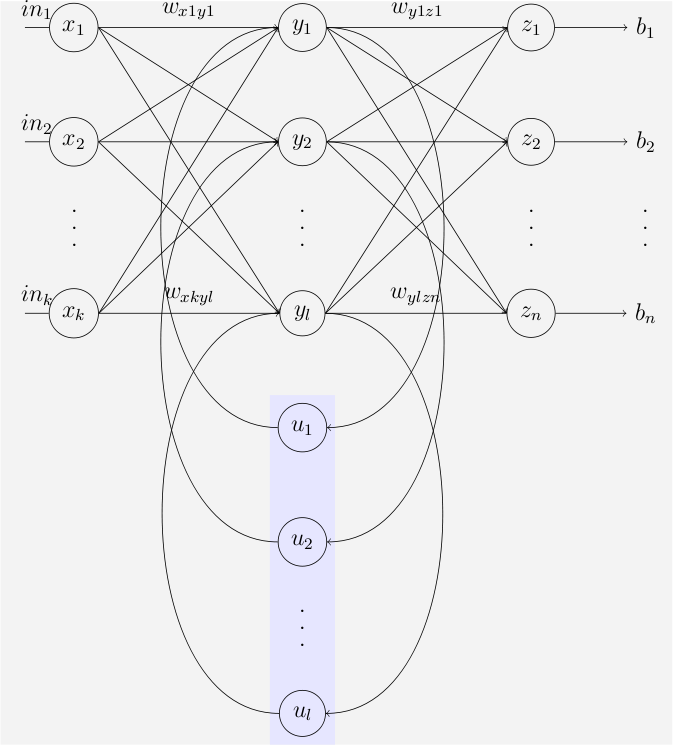
\includegraphics[scale=0.3]{elman.png}
        \caption{Representation of the Elman architecture}
    \end{figure} 
    The Elman architecture is a three-layer network, where the middle (hidden) layer is connected 
    to the context units(\textit{u} in the illustration) fixed with a weight of one. 
    At each time step, the input is fed forward and a learning rule is applied. 
    The fixed back-connections save a copy of the previous values of the hidden units in the 
    context units (since they propagate over the connections before the learning rule is applied). 
    Thus the network can maintain a sort of state, allowing it to perform such tasks as 
    sequence-prediction.
    The authors represent \textit{U}, \textit{W} and \textit{V} as the weight matrices of 
    the 3 layers, $w(t)$ as the input word at time \textit{t} on the form of \textbf{1-of-N encoding},
    $y(t)$ as the probability distribution function over semantic labels
    produced by the output layer and  $s(t)$ is used on the middle layer to maintain
    a representation of sentence history.
    \begin{align*}
        s(t) &= f(Uw(t) + Ws(t-1)) \\
        y(t) &= g(Vs(t)) \\
        f(z) &= \frac{1}{1 + e^{-z}} \\
        g(z_m) &= \frac{e^{z_m}}{\sum_k e^{z_k}}
    \end{align*} 
    The  model is trained using standard backpropagation to maximize the data 
    conditional likelihood.
    Then, the authors change the way words are encoded in the first layer to a bag-of-words,$x(t)$,
    in which there is a non-zero value for not just the current word, 
    but the next \textit{n} - 1 words as well and change the side information 
    of the network to dense vectors $f(t)$ instead of one-hot representations 
    via another hidden layer. The new hidden layer is connected to the middle one and the 
    output one and the connection weights are defined as \textit{F} and \textit{G} respectively.
    \begin{align*}
        s(t) &= f(Ux(t) + Ws(t-1) + Ff(t)) \\
        y(t) &= g(Vs(t) + Gf(t)) \\
        x(t) &= {w(t), w(t + 1)}
    \end{align*}
    Actually $x(t)$ can also be $w(t)$ or the defined bag of words vector.
   \newpage
   \subsubsection{Long Short-Term Memory Neural Networks}
   LSTM's are a type of RNN architecture with four layers, the \textbf{cell}, 
   the \textbf{input gate}, the \textbf{output game}, and the \textbf{forget game}.
   The cell remembers values over arbitrary time intervals and the three 
   gates regulate the flow of information into and out of the cell. 

    \newpage
    \medskip
    \bibliography{neural_networks_text_processing}
    \bibliographystyle{plain}
\end{document}